This report presents a length-based assessment of the multi-species deep slope fisheries targeting snappers, groupers, and emperors, as well as a number of other families, at depths ranging from 50 to 500 meters, in Fisheries Management Area (WPP) 573 in southern Indonesia. The most important fishing grounds in this area are located in the Indonesian part of the Timor Sea, near the edge of the Australian continental shelf.  There is also fishing around West Timor, Rote Island and other areas at the southern end of the Savu Sea, mostly by smaller scale operations. Surveys are ongoing to map other fishing grounds for these fisheries in WPP 573. Vessels operating in WPP 573 are originating from various ports throughout the country and may also operate in other WPP at times.

Gear types on target vessels include vertical drop lines and bottom set long lines at various scales, ranging from small scale village based fisheries with boats less than 5 GT to medium scale drop line and long line vessels measuring up to well over 100 GT for the largest long line vessels. The drop line fishery is an active vertical hook and line fishery operating at depths from 50 to 500 meters, whereas long lines are set horizontally along the bottom at depths ranging from 50 to 150 meters. The first year of this assessment (starting October 2014) includes only catches from drop line fisheries whereas long line catches were included from October 2015 onwards. This report analyzes length frequencies of the 50 most abundant species of fish that were caught by drop liners and long liners operating in WPP 573.  For a complete overview of the species composition please refer to the ID guide prepared for these fisheries:

\textbf{CLICK: }\href{http://72.14.187.103:8080/ifish/pub/TNC_FishID.pdf}{Link to on-line E-Book Species ID Guide}

For further background on species life history characteristics, and data-poor length based assessment methods, as applied in this report, please refer to the assessment guide that was separately prepared for these fisheries:

\textbf{CLICK: }\href{http://72.14.187.103:8080/ifish/pub/DeepSlopeSpeciesAssessmentTool.pdf}{Link to on-line E-Book Assessment Guide with Biological Information}

Since August 2015, all fish in the catch of cooperating vessels were photographed as they were caught. Fish were placed on top of measuring boards to enable sizing as well as identification from images. Photographs were taken by crew participating in our Crew Operated Data Recording System or CODRS. Images were analyzed by staff at our fisheries stations to generate species specific length frequency distributions that served as the input for length based assessments presented in this report.

Already since October 2014, fish landed at processing plants were measured there as part of a Smart Weighing and Measuring System (SWMS) intended to increase traceability and introduce species and size specific data collection in supply lines of target species. These data were also used in our length based assessments. The SWMS in processing plants captures length frequency data of fish that are processed in the facility, but the system does not record data on fish that are graded out beforehand. To capture the length frequency data also on batches of fish graded out before processing of the main catch, we developed a "mobile unit" or portable version of the SWMS which was used in ports like Kupang where parts of catches were offloaded to find their way to various traders and local markets. SWMS data were completed with these mobile unit data on those offloaded fish, to obtain more complete data sets on total catches. Data from our SWMS were used in the analysis up to October 2015, by which time they could be fully replaced with CODRS data on complete catches.

\begin{center}
\graphicspath{{/root/R-project/IFishSnapperWPP573/Images/}}
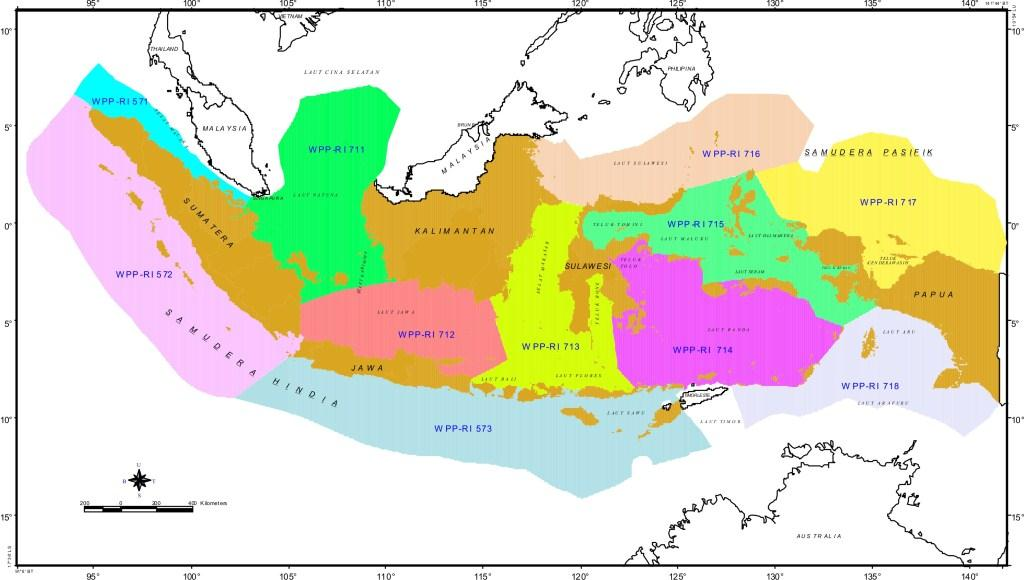
\includegraphics[scale=1.8]{wpp-indonesia.jpg}

Figure 1. Fisheries Management Areas (WPP) in Indonesian marine waters.
\end{center}

\begin{center}
\graphicspath{{/root/R-project/IFishSnapperWPP573/Images/}}
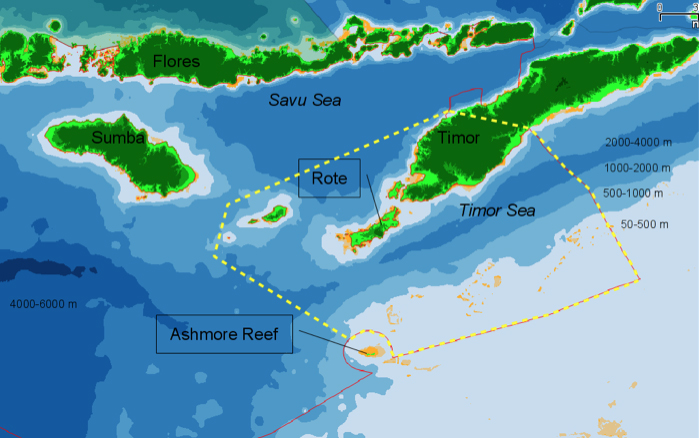
\includegraphics[scale=0.6]{timorsea.jpg}

Figure 2. The Indonesian part of the Timor Sea, bordering Australian waters.
\end{center}